\documentclass[12pt]{article}

%% preamble: Keep it clean; only include those you need

% if the below packages cannot be installed automatically, you can 
% download the required .sty files from CTAN and place them in the
% same location as the .tex file (or upload to overleaf in same
% location (folder) in overleaf

\usepackage{amsmath}
\usepackage[margin = 1in]{geometry}
\usepackage{graphicx}
\usepackage{booktabs}
\usepackage{natbib}

\usepackage{lineno}  % use these two lines to include line numbers
\linenumbers

\usepackage{setspace} % for doublespacing
\doublespacing


% highlighting hyper links
\usepackage[colorlinks=true, citecolor=blue]{hyperref}


\usepackage{color}
\newcommand{\blue}{\color{blue}} 
% when you make your edits in response to review/instructor comments, 
% you can indicate changes in color

%% meta data

\title{Stats Paper}
\author{Elizabeth Schifano\\
  Department of Statistics\\
  University of Connecticut
}

\begin{document}
\maketitle

\begin{abstract}
Here is the abstract.  Consult Note 4 on the course website for specific 
information about what should be included in these sections.  Also remember 
general \LaTeX guidelines and tips from Note 2. 
Include keywords at the end of the abstract section.\\

\noindent\textbf{Keywords}: keyword1, keyword2, keyword3.
\end{abstract}


\section{Introduction}
\label{sec:intro}

Use this section to answer three questions:
Why is the topic important/interesting?
What has been done on this topic in the literature?
What is your contribution?


To cite a reference, here are examples.
\citet{xie2015dynamic} did something ... 

Considerable work has already been published in this area 
\citep[e.g.,][]{xie2015dynamic}. Some parametric bootstrap sample size 
approach was proposed by \citet{dwivedi2017analysis}. 


% roadmap
The rest of the paper is organized as follows. The data will be presented in 
Section~\ref{sec:data}. Section~\ref{sec:meth} describes the methods. The 
results are reported in Section~\ref{sec:resu}. A discussion concludes in 
Section~\ref{sec:disc}.


\section{Data Description}
\label{sec:data}

Use this section to describe the data that helps to answer your research
questions. Some descriptive statistics in tables or figures are suggested 
here to summarize data.

Table~\ref{tab:rv} summarizes some distributional features for some of the 
variables in our dataset. $\ldots$

\begin{table}[!t]
  \caption{This is my first table.}
	\label{tab:rv}
\centering
\begin{tabular}{lrrr}
  \toprule
& Var 1 & Var 2 & Var 3 \\ 
  \midrule
Feature 1 & $-$0.110 & 4 & 2.401 \\ 
Feature 2 &    0.116 & 4 & 3.529 \\ 
Feature 3 & $-$0.066 & 6 & 11.104 \\ 
Feature 4 &    0.219 & 3 & 4.815 \\ 
Feature 5 &    0.303 & 5 & 2.188 \\ 
Feature 6 &    0.544 & 0 & 8.050 \\ 
Feature 7 & $-$2.617 & 8 & 3.646 \\ 
  \bottomrule
\end{tabular}
\end{table}


\section{Methods}
\label{sec:meth}

Use this section to present the methodologies that will generate results by
analyzing the data. 

Recall Einstein's equation
\begin{equation}
  \label{eq:mc2}
  E = m c^2,
\end{equation}
which states that the energy $E$ of a particle in its rest frame as the product
of mass ($m$) with the speed of light squared ($c^2$).

Suppose that the radius of a circle is $r$. Then its area is
\begin{equation}
  \label{eq:area}
  \pi r^2.
\end{equation}
%
Equation~\eqref{eq:area} is interesting, although it is short, and should not
be numbered (labeled) if it is not referenced elsewhere. It would likely be 
better as an inline expression, as in `Then its area is $\pi r^2$.' {\blue This 
text is in blue. It is sometimes helpful to highlight (in color) the changes 
that were made in response to reviewer's comments.}

Sometimes I don't want an equation to be numbered such as this one:
\[
  f(x) = \frac{1}{\sqrt{2\pi}} \exp\left( - \frac{x^2}{2} \right),
\]
which is the density of a standard normal variable.


\section{Results}
\label{sec:resu}

Report the results generated from the methods discussed in the previous section.  
Results can be from simulation and/or real data analysis.  

Figure~\ref{fig:cars} shows the distance against the speed from this dataset.

\begin{figure}[!t]
  \centering
  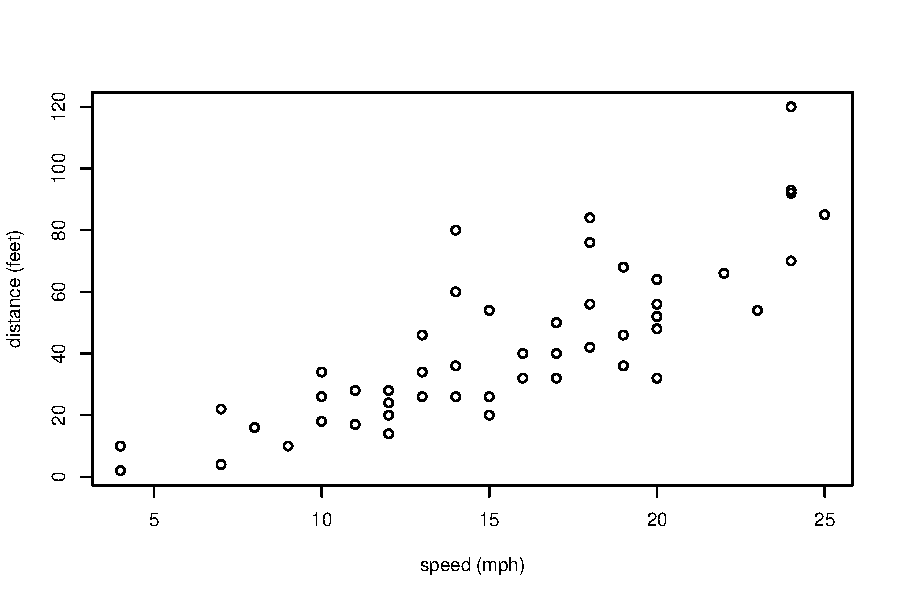
\includegraphics[width=\textwidth]{cars.pdf}
  \caption{This is my first figure.}
  \label{fig:cars}
\end{figure}

\section{Discussion}
\label{sec:disc}

What are the main contributions again?
What are the limitations of this study?
What are worth pursuing further in the future?
Blah, blah, blah.  Watch for prevalence of diabetes \citep{wild2004global}.

%\section*{Acknowledgements} %optional

\bibliography{refs}
\bibliographystyle{mcap}

%\section*{Appendix} %optional

\end{document}